\chapter{Configuración del Vocabulario}

El vocabulario no viene enteramente configurado en ATLAS Broadsea sino tan solo una pequeña demo adjunta a la base de datos de Eunomia, tal y como se describe en el repositorio de github de la \href{https://github.com/OHDSI/Broadsea-Atlasdb/tree/main}{ Base de datos de Broadsea}.

Por tanto, para poder utilizar ATLAS en profundidad se requiere la instalación y configuración del Vocabulario más extenso. OHDSI propone, en el repositorio de github de \href{https://github.com/OHDSI/Broadsea}{Broadsea} dos formas de configurar el vocabulario de Broadsea: (1) de forma manual (2) a través de Apache Solr. 

\section{Configuración manual}

La configuración manual del vocabulario requiere descargrar el vocabulario directamente desde ATHENA, instalarlo manualmente en el directorio local de Broadsea y ejecutar el contenedor docker encargado de montar el vocabulario en Broadsea. 


\subsection{Requisitos previos}

Para configurar el vocabulario manualmente,  se debe haber descargado el vocabulario y configurado el directorio local de Broadsea. Este procedimiento se ha seguido gracias al forum \href{https://forums.ohdsi.org/t/downloading-omop-cdm-version-5-vocabulary-data/3321/3}{Downloading OMOP cdm version 5 vocabulary data} y \href{https://forums.ohdsi.org/t/march-to-the-broadsea/20576}{March to the Broadsea}.

\begin{enumerate}

    \item Descargar el vocabulario desde la herramienta online de  \href{https://athena.ohdsi.org/}{ATHENA}.Para ello, acceder al menú de descarga \code{Download}. En este momento se presenta un listado de todos los vocabularios que contiene ATHENA entre los que algunos aparecen preseleccionados. Cada usuario puede seleccionar o deseleccionar los vocabularios que le interesen para el estudio que esté realizando. En este caso, se descargará el vocabulario que ATHENA sugiere por defecto.
    
    \begin{figure}[H]
        \centering
        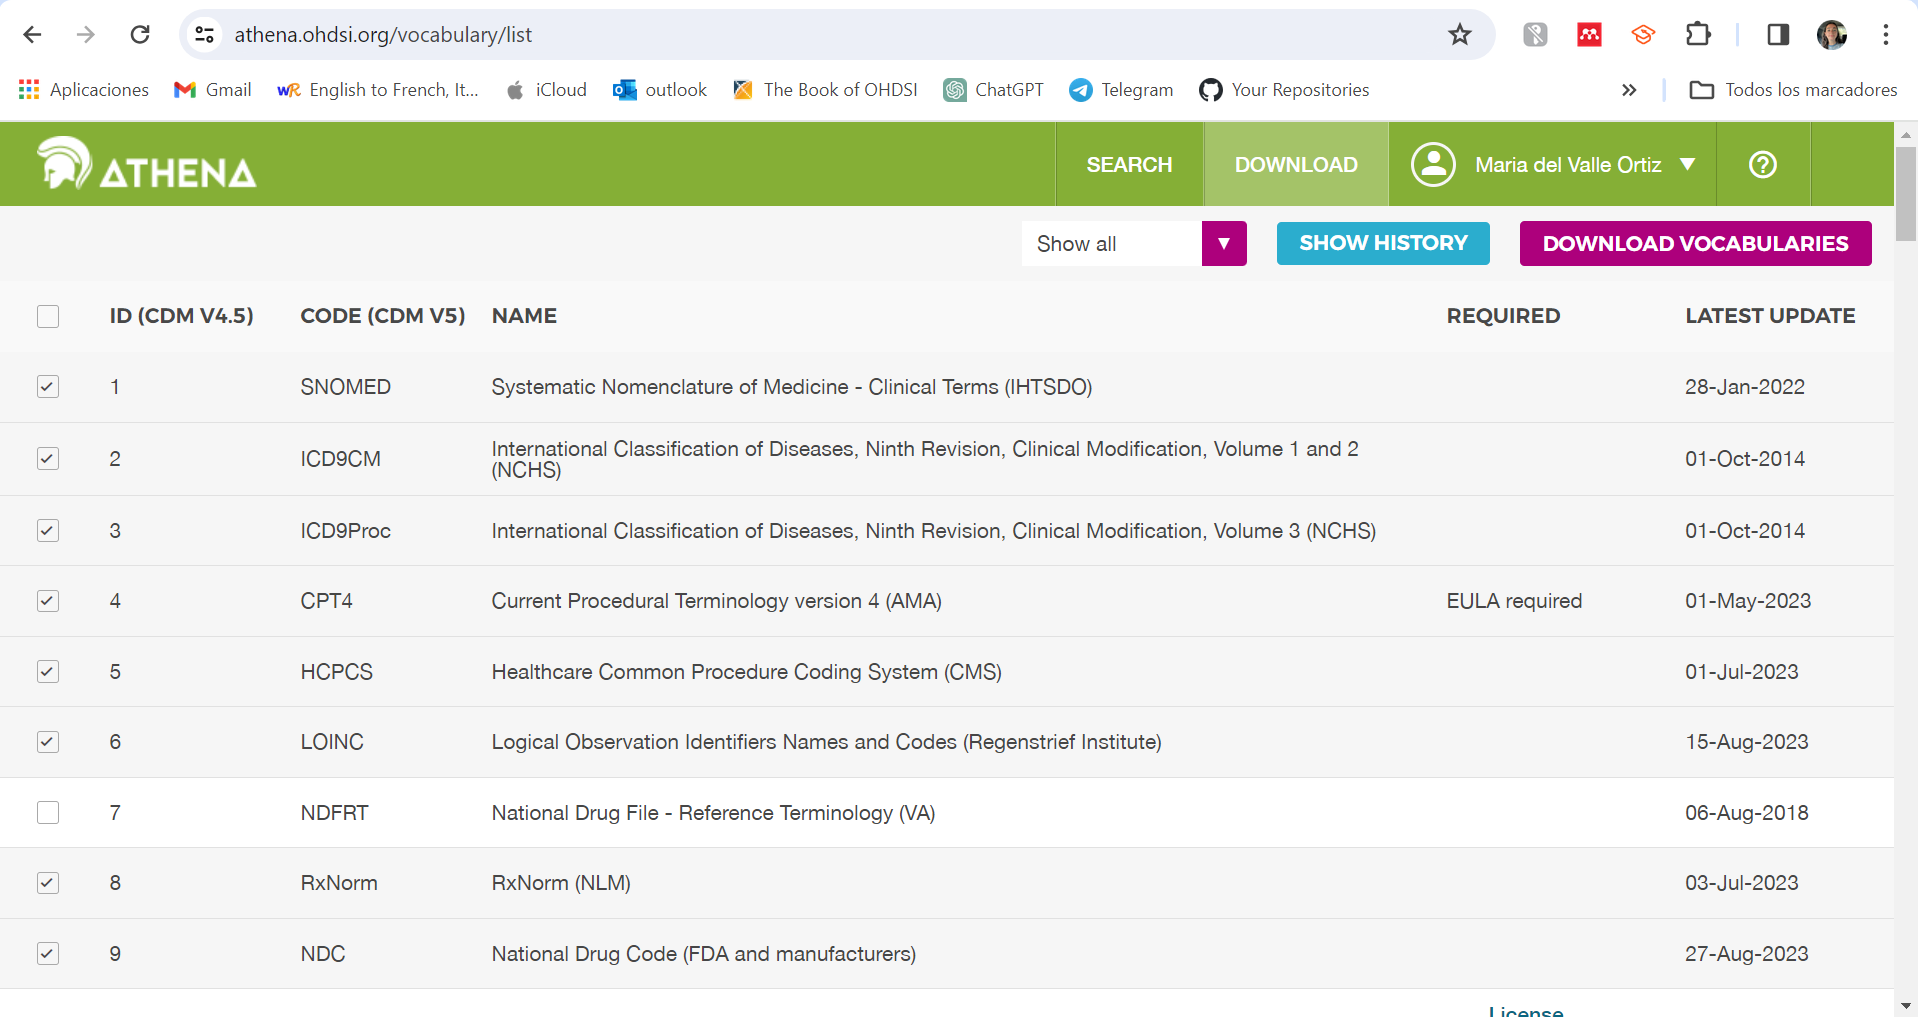
\includegraphics[width=0.90\textwidth]{figures/athenaPreDownload.png}
        \caption{Captura de pantalla de la preselección de vocabularios para descargar.}
        \label{fig:athenaPreDownload}
    \end{figure}

    \item La descarga requiere registrar un usuario con un correo electrónico válido al que se enviará un link personal que permitirá la descarga de un archivo .zip con el vocabulario seleccionado. También desde ATHENA en la pestaña \code{SHOW HISTORY} muestra el estado en el que se encuentra la descarga del vocabulario y, una vez que esté listo, permite la descarga directa del zip.

    \item El archivo zip que se descarga, una vez descomprimido, muestra varios archivos .csv con las tablas que conforman el Vocabulario y otros archivos CPT4 que no serán de interés. 

      \begin{figure}[H]
        \centering
        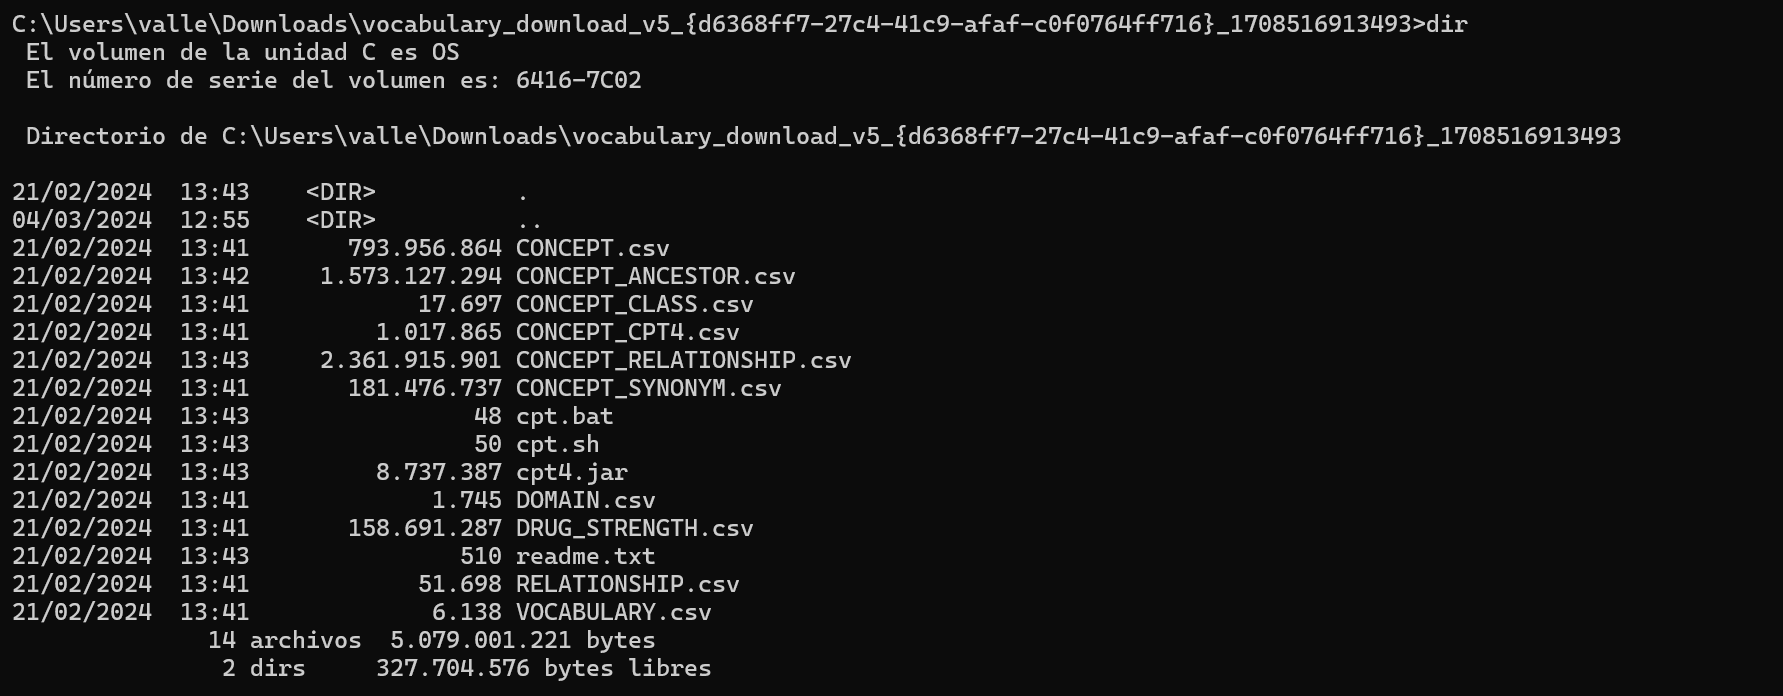
\includegraphics[width=0.90\textwidth]{figures/vocabDownload.png}
        \caption{Captura de pantalla de archivos descargados del vocabulario.}
        \label{fig:vocabDownload}
    \end{figure}

    \item Por último, los archivos descargados del vocabulario deben almacenarse en el directorio local de Broadsea, concretamente en la ruta \code{Broadsea/omop\_vocab/files}. En caso de no existir la carpeta \code{/files}, crearla manualmente. Este paso es muy importante.

\end{enumerate}

\subsection{Deployment}

Configurar el vocabulario requiere establecer una configuración avanzada del contenedor Docke de Broadsea. Si bien, la primera vez que se inicializó el contenedor se ejecutó el perfil \code{default} ahora se va a ejecutar específicamente el perfil \code{omop-vocab-pg-load}. Esta opción se especifica en la sección \href{https://github.com/OHDSI/Broadsea?tab=readme-ov-file#omop-vocab-loading}{OMOP Vocab Loading} del repositorio de Broadsea. También ha sido de utilidad el mismo forum \href{https://forums.ohdsi.org/t/march-to-the-broadsea/20576}{March to the Broadsea}.

Para acceder a la información y configuración avanzada del perfil se puede acceder al \code{docker-compose.yml} y a la sección 9 del archivo \code{.env}, aunque este caso no será necesario realizar ninguna modificación sobre los mismos.

\begin{enumerate}

    \item Para comenzar la configuración del vocabulario es necesario inicializar el contenedor \code{omop-vocab-load}. Ejecutar la siguiente línea de código en el \code{cmd}:

    \begin{lstlisting}[language=sh]
    docker compose --profile omop-vocab-pg-load up -d\end{lstlisting}

    Este comando da lugar el siguiente resultado.

      \begin{figure}[H]
        \centering
        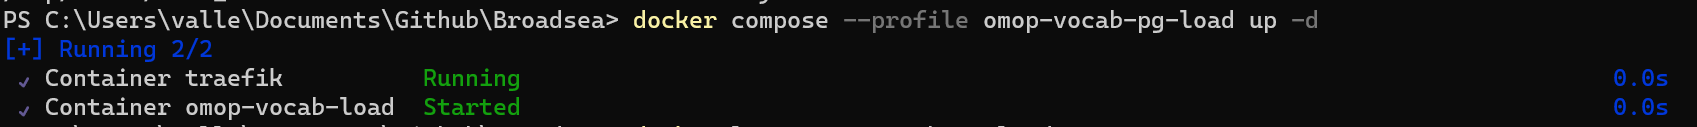
\includegraphics[width=0.90\textwidth]{figures/composeProfVocabLoad.png}
        \caption{Captura de pantalla de comando para iniciar el perfil docker.}
        \label{fig:composeProfVocabLoad}
    \end{figure}

    \item Durante la instalación del contenedor es muy importante tener abierto el \code{logs} de Docker. Se recomienda abrirlo desde Docker en vez de desde el \code{cmd} porque este último imprime el \code{logs} que se ha ejecutado hasta el momento en que se ejecuta el comando, no mantiene abierto el \code{logs} hasta que el contenedor se termine de inicializar. Sin embargo, Docker sí muestra el control en tiempo real del proceso. Proceso que ha durado 2h.

    \item Una vez que el proceso finaliza correctamente, se imprime un mensaje en el log que advierte que el contenedor puede ser eliminado y el estado del contenedor pasa a ser \code{Exited}. A continuación se presenta una captura de pantalla de las últimas líneas de dicho log.

 \begin{figure}[H]
        \centering
        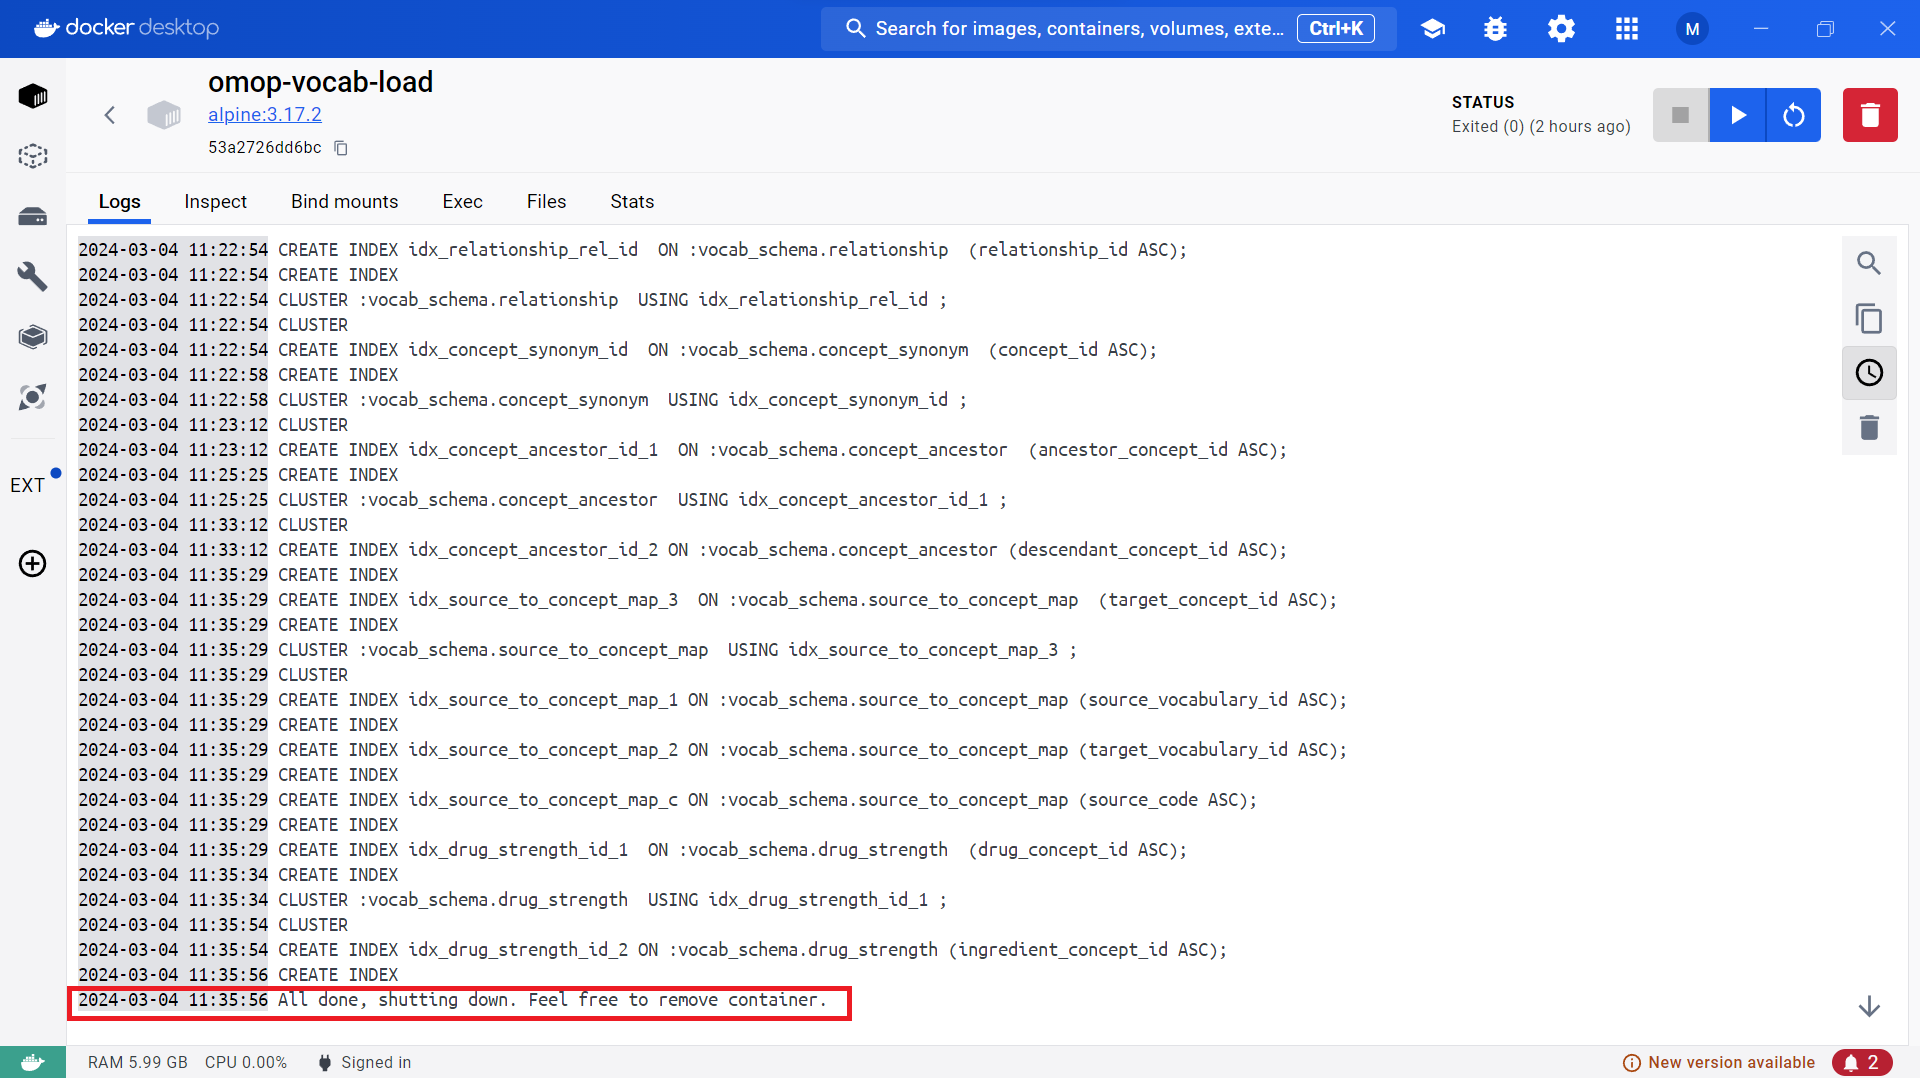
\includegraphics[width=0.90\textwidth]{figures/vocabLoadLogSuccess.png}
        \caption{Captura de pantalla de log de instalación exitosa del perfil docker.}
        \label{fig:vocabLoadLogSuccess}
\end{figure}
    
    
\end{enumerate}

\subsection{Compobación de configuración correcta}

Para comprobar que se ha configurado correctamente el vocabulario en la base de datos de Broadsea, se puede (a) consultar el administrador de la base de datos y (b) realizar una búsqueda en ATLAS.

\begin{enumerate}

    \item La comprobación consultando el administrador de la base de datos implica abrir pgAdmin, acceder al servidor y a la base de datos de Broadsea y revisar el listado de esquemas. Debe aparecer un nuevo esquema denominado \code{omop\_vocab}.
    
    A continuación, para comprobar que el esquema se haya instalado completamente, se puede seleccionar cualquiera de las tablas que lo componen, click derecho \code{View data/All rows} y comprobar que la tabla no esté vacía. En este ejemplo se ha utilizado la tabla \code{vocabulary} para realizar la comprobación.

 \begin{figure}[H]
        \centering
        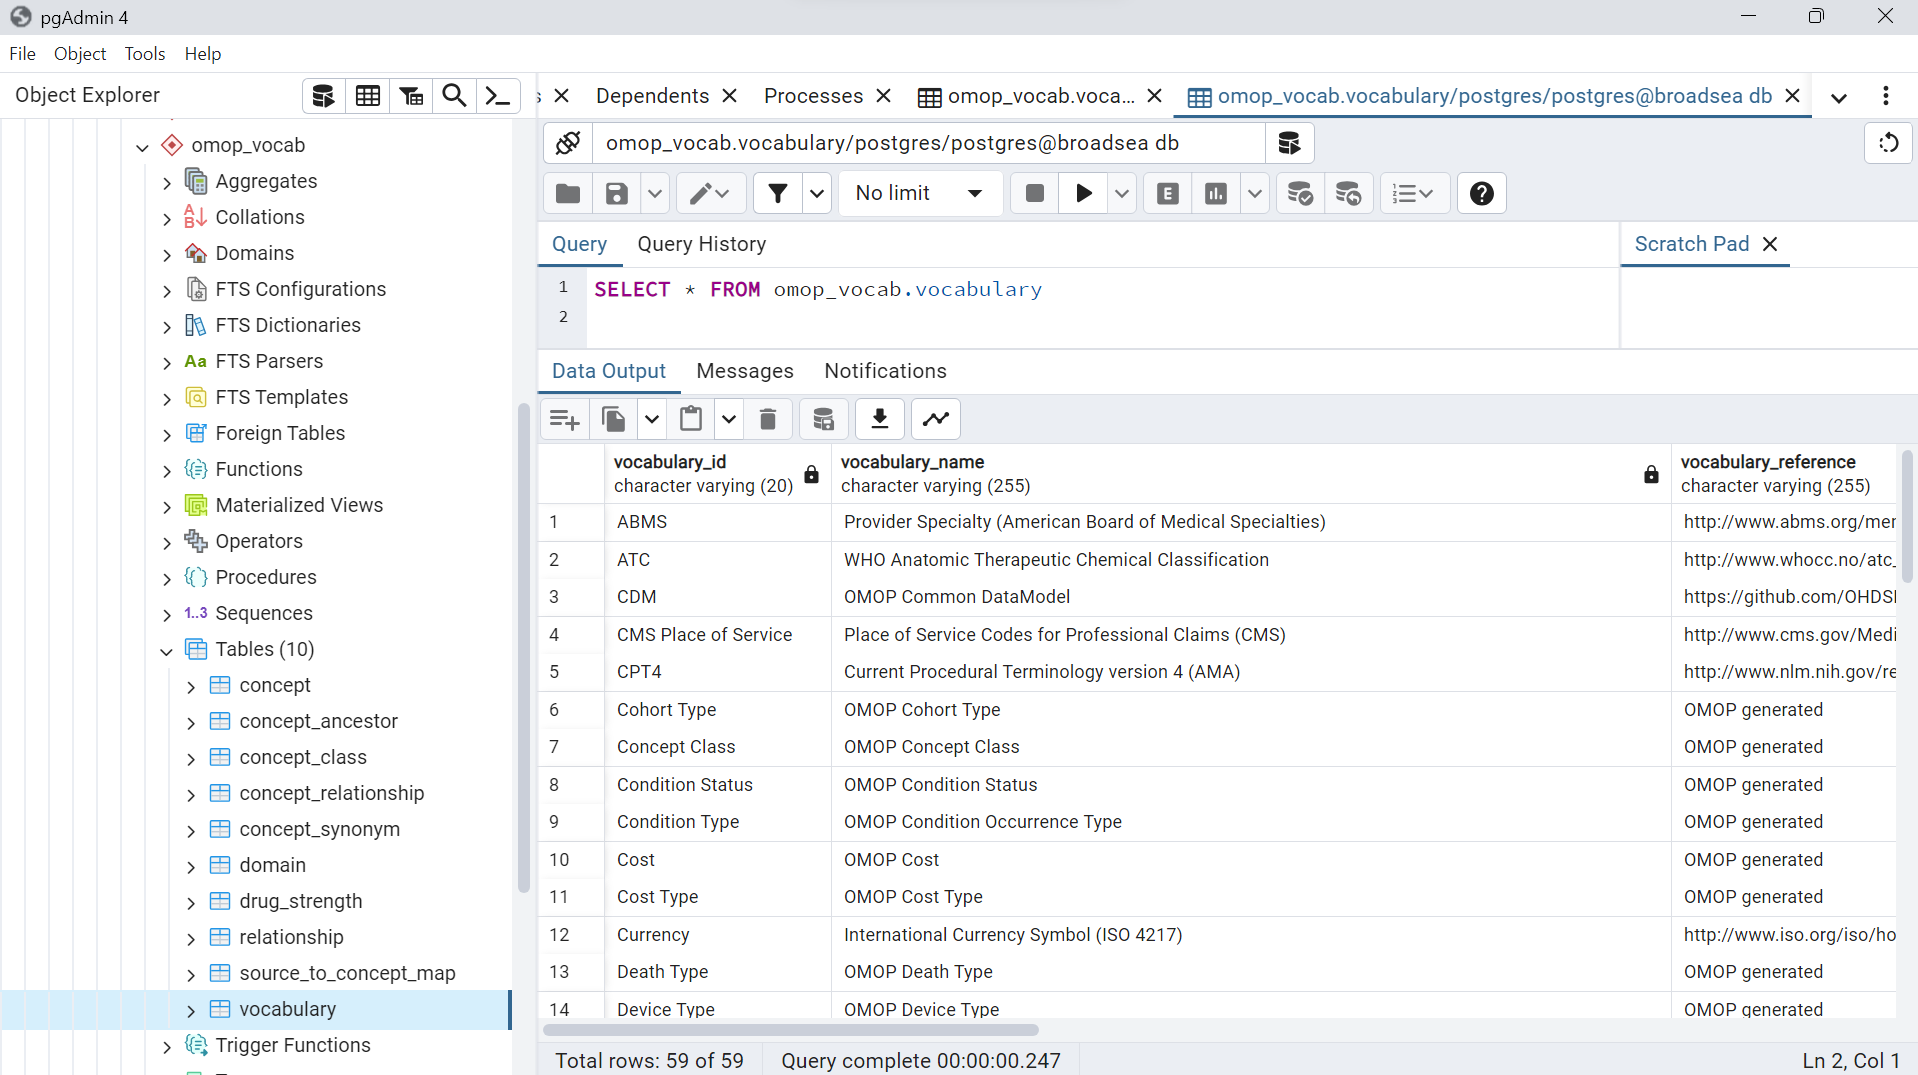
\includegraphics[width=0.90\textwidth]{figures/omopVocabComprobacion.png}
        \caption{Captura de pantalla de comprobación de configuración correcta del vocabulario en pgAdmin.}
        \label{fig:omopVocabComprobacion}
\end{figure}

    \item Otra opción es realizar un búsqueda en ATLAS
    
\end{enumerate}

\subsection{Solución de posibles errores}

- No haber creado la carpeta /files

- Haber creado la carpeta /files pero vacía

- Se crea el esquema pero se queda vacío: ESPERATE A QUE SE EJECUTE EL CONTENDOR 

\section{Configuración mediante Apache Solr}

- Se ha intentado. No se ha podido.. Está bajo desarrollo aún.

- Issue en github y forum.

